\gls{idpcdu} can be briefly stated as follows: Given a finite set of colors $D$ and a weighted directed multi-graph $G=(V, E, w, s, t)$, where $V$ and $E$ are the set of nodes and the set of domains, respectively. Each edge $e \in E$ is assigned a positive weight $w(e) \geq 0$ and a color $d \in D$, which represents a network domain. Let $E^d$ be the set of $d$-colored edges. Therefore, $E^d$ is a partition of $E$, or in general, each edge belongs to one specific domain. \gls{idpcdu} searches for a min-cost feasible path $p$ from the source node $s$ to the target node $t$, and specifically, $p$ traverses every domain at most once according to the \gls{du}.

\begin{center}
	%	\begin{tabular}{l p{5.5cm}} %<----2 cot
	\begin{tabular}{lp{10cm}}
		\hline 
		\textbf{Input}:	&- A weighted directed multi-graph 
		$G = (V, E, w, s, t)$,\\
		&- $E$ is partitioned into $D$ domains $\{E^1, E^2, . . ., E^{|D|}\}$, $E^i \cap E^j = \emptyset$.\\
		&  - A source $s$ and a target $t$.\\
		\hline
		\textbf{Output}: &  A path $p = \{p_0,~p_1,\dots,~p_h\}$, $p_i \in E$ $\forall i$, $p_0 = s,~p_h = t$\\
		\hline 
		\textbf{Constraint}: & \gls{du}: Once $p$ has left a domain, it is not allowed to revisit it later on. If $p_{i} \in E^d$ and $p_{i+1} \notin E^d$, $p_{i+k} \notin E^d$  $\forall k\geq2, 1\le d \le |D|, p_i \in E$. \\
		\hline 
		\textbf{Objective}: & $\displaystyle \sum_{i =0 }^{h-1} w(p_i,p_{i+1}) \rightarrow $ minimum.\\
		\hline 
	\end{tabular}
\end{center}
\bigskip
An example of the input multi-graph $G$ for \gls{idpcdu} is depicted in Figure~\ref{fig:input_graph}. In this case, $G$ contains eight nodes, and its set of edges is separated into four domains, namely $red,~blue,~green$, and $grey$. \gls{idpcdu} determines the optimal path from source node $s$ to the target one $t$ such that the \gls{du} is fulfilled. Figure~\ref{fig:valid_path_a} illustrates a valid solution, which traverses only three out of four domains. Conversely, two possible invalid ones are shown in Figure~\ref{fig:invalid_path_b} and~\ref{fig:invalid_path_c}. The first is a path that violates the \gls{du} by re-entering the $red$ domain twice. The other case occurs when a path visits a node of no out-edge, thus unable to reach $t$.
\bigskip
\setlength{\intextsep}{3pt}
\renewcommand{\scalefigure}{0.7}
\begin{figure}[htbp]
	\centering
	\begin{subfigure}{.49\linewidth}
		\centering
		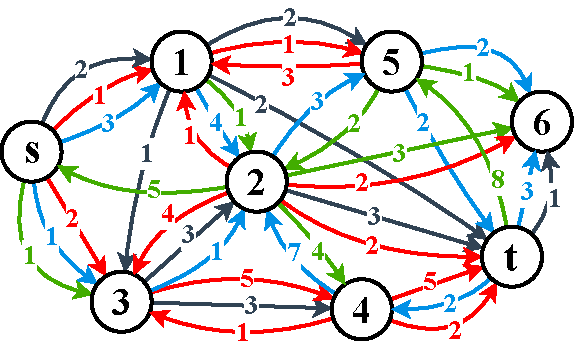
\includegraphics[scale=\scalefigure]{Figures/chap 2/Bold Input Graph.pdf}
		\caption{An input graph}
		\label{fig:input_graph}
	\end{subfigure}
	\begin{subfigure}{.49\linewidth}
		\centering
		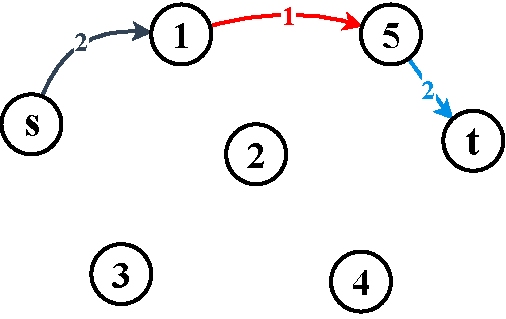
\includegraphics[scale=\scalefigure]{Figures/chap 2/Valid Solution.pdf}
		\caption{A valid solution}
		\label{fig:valid_path_a}
	\end{subfigure}
	\begin{subfigure}{.49\linewidth}
		\centering
		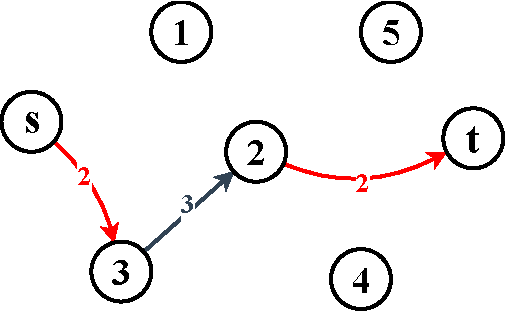
\includegraphics[scale=\scalefigure]{Figures/chap 2/Invalid Solution.pdf}
		\caption{An invalid solution that violates the \gls{du} constraint}
		\label{fig:invalid_path_b}
	\end{subfigure}
	\begin{subfigure}{.49\linewidth}
		\centering
		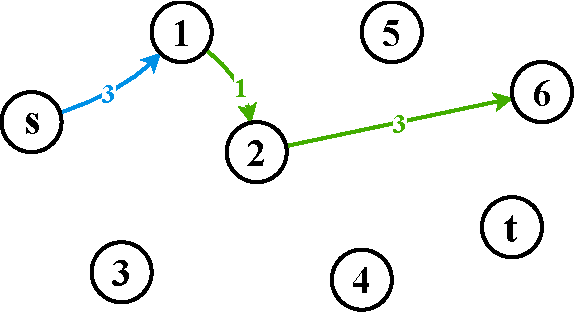
\includegraphics[scale=\scalefigure]{Figures/chap 2/Invalid Solution 2.pdf}
		\caption{An invalid solution that can not reach
			the target node}
		\label{fig:invalid_path_c}
	\end{subfigure}	
	\caption{An example input graph and solution cases for \gls{idpcdu}}
	\label{fig:solution_cases}
\end{figure}